% !TEX root = ../notes.tex

% ================  (Interactive) Visualization ==============

\section{Supervised Learning}
 
\subsection{Machine Learning}
We give the difference between Supervised and Unsupervised Learning before going deeper into the Supervised Learning.
\href{http://www.r2d3.us/visual-intro-to-machine-learning-part-1/}{Beautiful Introduction to Machine Learning!} -> Introduce main concepts used in this course.
\\
Machine LEarning is born because we are \textbf{lazy}! So, we let the machine ``work'' for us.


\textbf{Supervised} 
\\\\
Input and output samples $(X,y)$ are given. They are linked together with a functions $f$ such that $f(X) = y$. The idea is \emph{learn} $f$ and evaluate it on new data. We can find two different types:
\begin{itemize}
 \item \textbf{Classification}: y is a discrete value.
 \item \textbf{Regression}: y is continuous (e.g. linear regression)
\end{itemize}
Examples:
\begin{itemize}
 \item Is this image a cat, dog, car, house?
 \item How would this user score that restaurant?
 \item is this email spam?
 \item Is this blob a supernova?
\end{itemize}
Techniques:
\begin{itemize}
 \item kNN (k Nearest Neighbors)
 \item Na\"ive Bayes
 \item Linear + Logistic Regression
 \item SVM (Support Vector Machines)
 \item RF (Random Forests) + GRD (Greedy Random Forests)
 \item Neural Networks
 \item etc.
\end{itemize}

\textbf{Unsupervised}
\\\\
We only get samles $X$ of the data and we want to compute a function $f$ to create a \emph{simple representation} given by $y = f(X)$. We can also differenciate between discrete and continus:
\begin{itemize}
 \item y is \textbf{discrete} corresponds to clustering.
 \item y is \textbf{continuous} corresponds to Matrix factorization, Kalman filtering, unsupervised neural networks. 
\end{itemize}
Examples:
\begin{itemize}
 \item Cluster some hand-written digit data into 10 classes
 \item What are the top 20 ropics in Twitter right now?
 \item Find and cluster distinct accents of people in Lausanne. 
\end{itemize}
Techniques:
\begin{itemize}
 \item Clustering
 \item Topic Models
 \item HMMs (Hidden Markov Models)
 \item etc.
\end{itemize}

\subsection{More details on Supervised Learning}

\subsubsection{Predicting from Samples}

Most of the datasets are \textbf{samples} from an infinite population, \emph{i.e.} a subset of an \textbf{infinite} dataset. We would like to model the \textbf{whole population}, but only have access to a sample of it. So, we train on a training sample called $D$ and we denote the model as $f_D(X)$ where $X$ are the features and $y=f_D(X)$ the predictions.

\subsubsection{Bias and Variance}

The data-generated model $f_D(X)$ is a \textbf{statistical estimate} of the true function $f(X)$ (function working for the whole population). Therefire, the model is subject ot bias and variance. 
\\
The \textbf{Bias} is defined as the \emph{expected difference} between the prediction of a model $f_D(X)$ and the true labels $y$:
\[
 \textrm{Bias} = \mathbb{E}\left[ f_D(X)-y\right]
\]
\\
The \textbf{Variance} is defined as:
\[
 \textrm{Variance} = \mathbb{E}\left[\left(f_D(X) - \overline{f}(X)\right)^2\right]
\]
where $\overline{f}(X) = \mathbb{E}\left[f_D(X)\right]$ being the average prediction on X.

Bias and Variance are very useful to understand if you're doing something wrong. So, try to understand what you're doing and not just applying ``black-boxed'' algorithms.
\\\\
\textbf{Tradeoff between Bias and Variance}
\\
Tradeoff between bias and variance due to model complexity:
\begin{itemize}
 \item \textbf{Complex models}: Many parameters, usually lower bias but higher variance
 \item \textbf{Simple models}: Few parameters, higher bias but lower variance.
\end{itemize}

For example, a linear model can only fit a straight line. A high degree polynomial can fit complex curves => this one will work very well with the sample but not that well with the population => high variance!
\\\\
The total expected error is 
\[
 \textrm{Bias}^2 + \textrm{Variance}
\]
Because of the bias-variance tradeoff, we want to \textbf{balance} their contributions. \emph{Variance} dominates => \textbf{over-fitting}. \emph{Bias} dominates => \textbf{under-fitting}.

\subsubsection{k-Nearest Neighbors}
Issues: \\
Data \textbf{is} the model. => no training needed, accuracy improves with more data. Matching is simple and fairly fast if data fits in memory. It usually needs data in memory, but can be run off disk. 
\\\\
Min config: \\
There's only one parameter: $k$, the number of neighbors. But two other choices are important:
\begin{itemize}
 \item Weighting of neighbors (inverse distance)
 \item Similarity metric.
\end{itemize}

\textbf{k-NN Flavors}
\\\\
TO PUT IN A TABLE \\
Classification:
\begin{itemize}
 \item Model is $y=f(x)$, y the labels (discrete set)
 \item Given X, compute y (= majority vote of the k nearest neighbors.
 \item Can also use a weighted vote* of the neighbors
\end{itemize}
Regression:
\begin{itemize}
 \item Model is $y=f(x)$, y is a real value
 \item Given X, compute y = average value of the k nearest neighbors
 \item Can also use a weighted average* of the neighbors.
\end{itemize}
\textbf{k-NN distance measures}
\\\\
\begin{itemize}
 \item Euclidean distance
 \item Cosine Distance
 \item Jaccard Distance
 \item Hamming Distance
\end{itemize}
\textbf{k-NN metrics}
\\\\
\begin{itemize}
 \item Manhattan distance
 \item edit distance
 \item Mahalanobis distance
\end{itemize}
\textbf{Choosing k}
\\\\
Small k -> low bias, high variance \\
Large k -> high bias, low variance \\
\\\\
\textbf{In practice}
\\
Use cross-valid! (Training for 80\% and testing for 20\%) \\
Predict: For each point in the validation set, predict using the kNN from the training set. Measure the error rate(classification) or the squared error(reg). \\
Tune: try different values of k and use the one that gives min error. \\
Evaluate: Test on the test set to measure performance. \\\\
\textbf{kNN and the curse of dimensionality} 
\\\\
\textbf{curse of dimensionality} refers to phenomena that occur in high dimensions (100 to millions) that do not occur in low dimensional-space. In particular, data in high dimensions are much sparser than data in low dimensions. For kNN, that means there are less points that are very close in feature space (similar) to the point we want to predict. [EXAMPLE] => surprising that kNN in high dimension. Luckily real data are not like random points in a high dimensional cube. => live in \textbf{dense clustes} and near \textbf{much lower-dimensional surfaces}. Finally, points can be very ``similar'' even if their euc distance is large.

\subsection{Decision tree}

Classification <-> training. We can try 1 classifier per each section. \\
Training : Categorical attributes, numerical attributes and class label. The we use a classification algorithm and create the model (classifier). \\\\
\textbf{Characteristics of classification methodes} 
\\\\
Predictive accuracy \\
Speed and scalability (time to build the model, time to use it, in memory vs disk processing) \\
Robustness: (Handling noise, outliers and missing values) \\
Interpretability: (Understanding the model and its decisions [black vs white box], compactness of the model) \\
\textbf{Decision tree induction} 
\\\\
Model: flow-chart like tree structure:
\begin{itemize}
 \item Nodes are test on a single attribute
 \item Branches are attribute values
 \item Leaves are marked with class labels
\end{itemize}
Score function: classification accuracy \\
Optimisation: top-down tree construction \\
Tree construction:
\begin{itemize}
 \item at the beginning, All training samples belong to the root
 \item Examples are partitioned recursively based on selected ``most discriminative'' attributes
 \item discriminative power based on information gained
\end{itemize}
Partitioning stops if 
\begin{itemize}
 \item All samples belong to the same class -> assign the class label to the leaf
 \item There are not attributes left -> majority voting to assign the class label to leaf
 \item THere are no samples left
\end{itemize}
\textbf{Attribute selection}
\\\\
At a given branch in the tree, the set of samples $S$ to be classified has $P$ positive and $N$ negative samples. The amount of entropy in the set $S$ is:
\[
 H(P,N)=-\frac{P}{P+N}\log_2\frac{P}{P+N}-\frac{N}{P+N}\log_2\frac{N}{P+N}
\]
Note that:
\begin{itemize}
 \item If $P=0$ (or $N=0$), $H(P,N)=0$ => no uncertainty
 \item If $P=N$, $H(P,N)=1$ => max uncertainty
\end{itemize}
{\huge \color{red} TO FINISH WITH THE SLIDES OF THE COURSE}




%========================================
\subsubsection{Random Forest}

A common problem when trying to build a model is to select significant features between all the available one. We tend to think that \textit{the more we have, the better it is}, even knowing the existence of the curse of dimensionality. 

Random Forest takes this idea and try to automatize this feature selection by randomly selecting subset of features.

The main idea of Random Forest algorithm is to grow an arbitrary number of \textbf{Decision Trees}, each one grown based on a subset of m features, randomly chosen between the total $p$ of them. It's an example of a \textbf{weak learner} saw in the Ensemble method. This weak learner has a lower bias (because of lower number of feature).

Following the \textbf{Ensemble method}, the predictions of all these weak learners are then merged together to produce a final prediction (by majority voting for example).



\begin{center} %---------------TAB--------------
\begin{tabular} {| l | l |}
\hline
\bf Pros & \bf Cons \\ \hline
+ Popular & - Not state-of-the-art  \\
+ Easy to implement & - Needs many passes over the data \\
+ Easy to parallelize & - Tend to overfit \\ 
\hline
\end{tabular}
\end{center}

\subsubsection{Boosted Decision Trees}
Variante of Random Forest. Instead of training all DT independently on weak subset, the DT are trained sequentially and emphase incorrectly-labeled instances of the previous tree. This is called \textbf{Boosting}. 
\begin{itemize}
\item Low variance, because of the small trees handling small numbers of features
\item Low bias, reduces by the boosting
\end{itemize}

Opposed to RF that usually trained tens of medium-sized trees, BDT works on smaller trees in greater numbers.

Even if they show good results, their big drayback is their slow execution compared with the parallelized RF.


\subsubsection{About model transparency}

A recurrent argument of using Decision Tree (DT) or Random Forest (RF) in industry is their transparency compared to state-of-the-art Deep-Neural-Network (DNN). This argument must be carefully taken. Even if by their very nature DT are more understandable by a human than DNN, the more features and Trees we had, the more complicated it becomes. Figure \ref{pic:RF_BT} shows the size of a common industry implementation of RF and BT where there are no more possibilities of human understanding.

\begin{figure}[H]%---------------FIG--------------
 \centering
 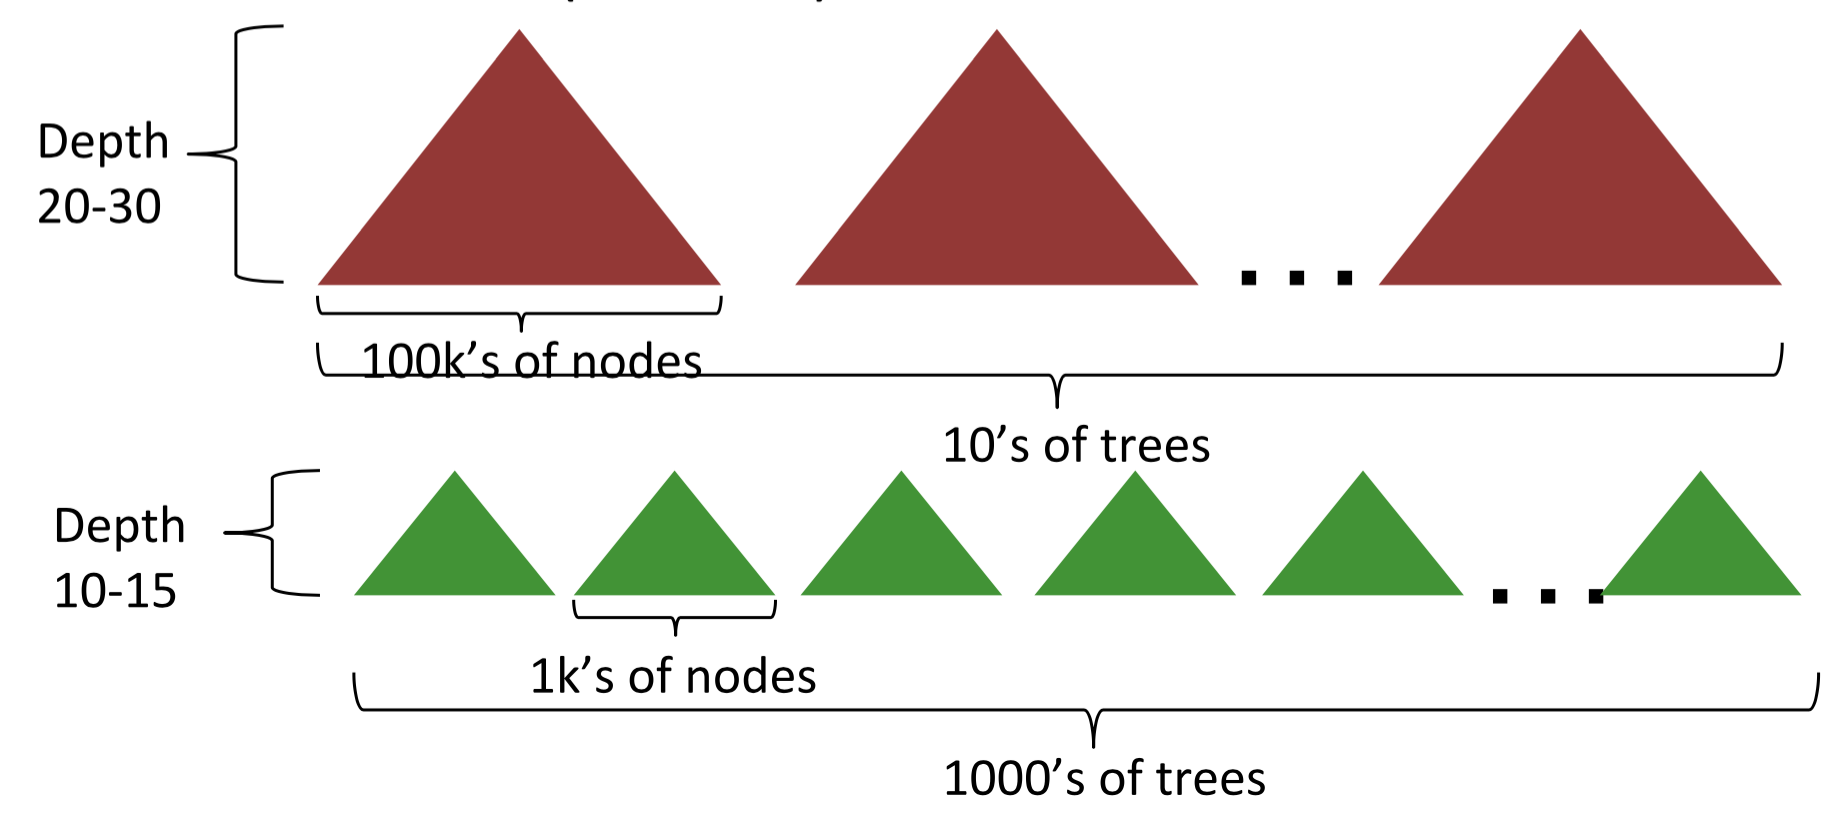
\includegraphics[width=10cm]{./img/07/RF_BT.png}
 \caption{\label{pic:RF_BT.} Standard size of RF and BDT implementations.
 In red: RF with big parallel DT. In green: BDT pipeline with lot of small DT}
\end{figure}


\subsection{Linear Regression}

Linear regression model produces a prediction equation:

$$
\hat{y} = \hat{\beta_0} + \sum\limits_{j=1}^p  X_j + \hat{ \beta_j}
$$

or in matrix notaction

$$
\hat{y} =X \hat{ \beta}
$$

Where $X_j$ are the data and $\hat{\beta_j}$ the characteristic of the model. 

\subsubsection{Statistic validation}

As a linear model can be calculated for every possible existing dataset, it is not enough to calculate it, but the existing of linear relationship between the data must be prooved.

\paragraph{$R^2$-value}

$R^2$-value describes how much of the total variance is reduced when we include the line as an offset. It computes the distances between the real $y$ and the predicted $\hat{y}$, and compares them with the distance between real $y$ and the mean $\bar{y}$.

\begin{itemize}
\item if $R^2 = 0$, then there is no difference between the linear model and the trivial mean $\bar{y}$. Then we conclude that there is not any evidence of linear relationship in our dataset and \textbf{we cannot use the model}.
\item if $R^2 = 1$, then the data perfectly alligned on the linear regression line and \textbf{the model is perfect}.
\end{itemize}

\begin{figure}[H]%---------------FIG--------------
 \centering
 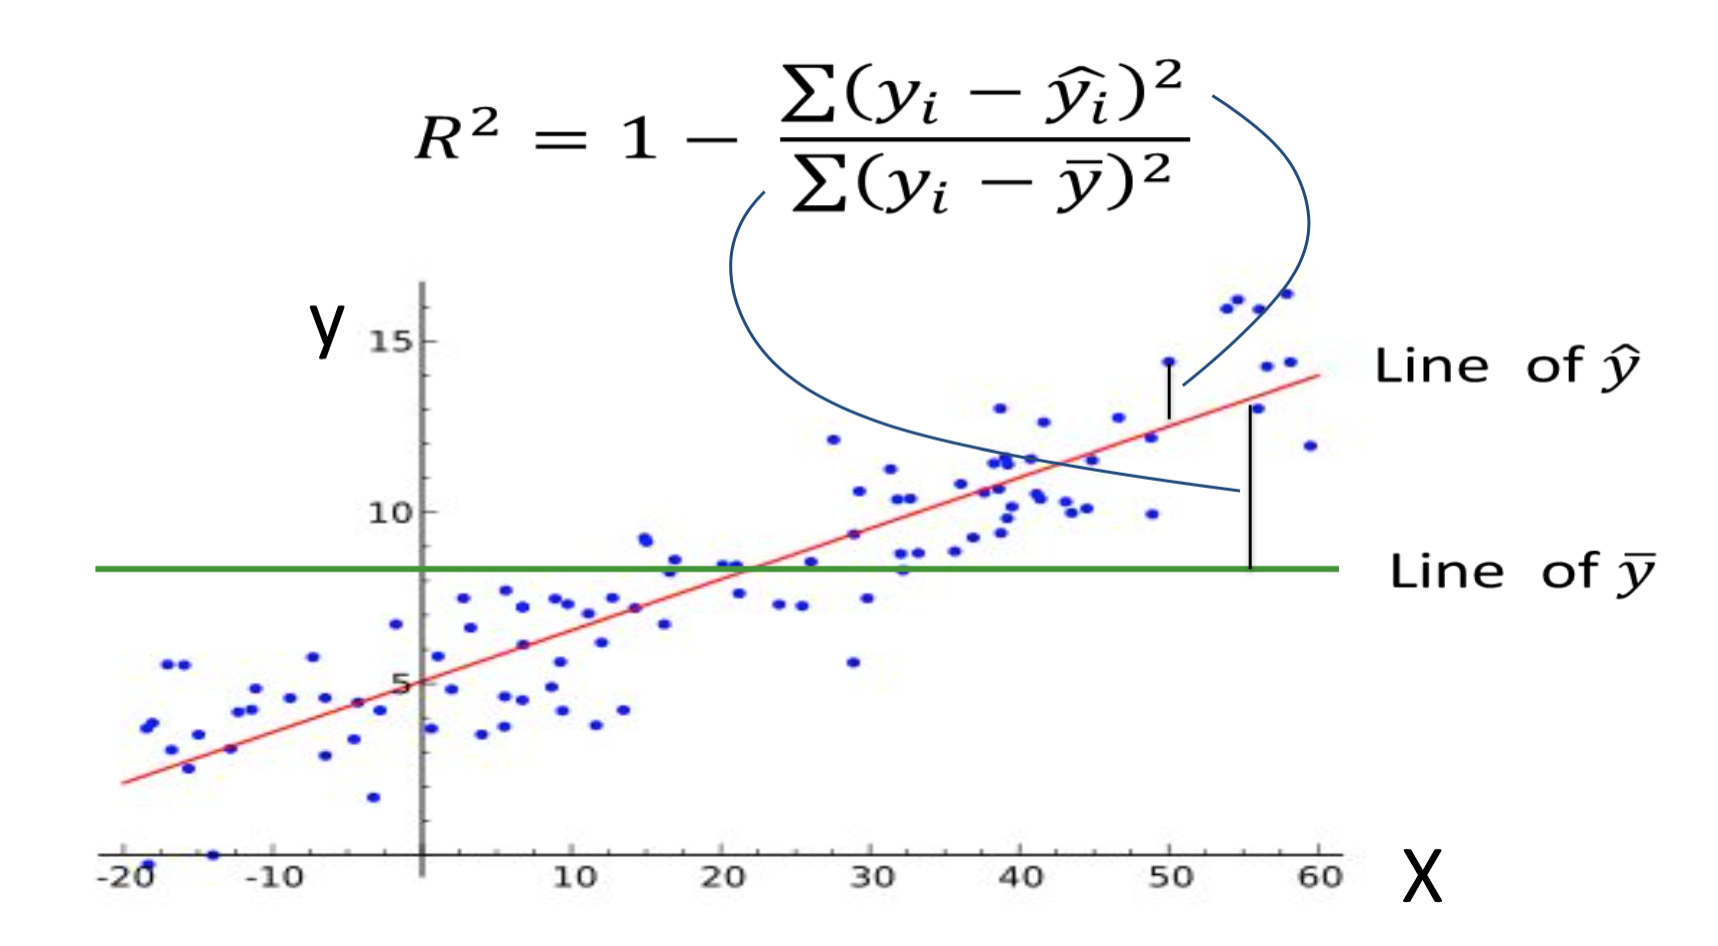
\includegraphics[width=10cm]{./img/07/r_2.png}
 \caption{\label{pic:r_2} Graphical meaning of $R^2$-value.}
\end{figure}


\paragraph{p-value}

From the Distribution of Fisher (F-Distribution) we can derive a p-value which is, as usual, the probability that the observed data are produced by the null hypothesis which is, in our case, the hypothesis \textit{no linear relationship}. For $p < 0.05$ we conclude, as usual, that it is very unlikely that the data were produced by the null hypothesis and we then accept the hypothesis \textit{the data are produced by linear relationship}.














